% Capítulo 11: o ciclo de depuração.
\documentclass[border=4pt]{standalone}
\usepackage[utf8]{inputenc}
\usepackage[T1]{fontenc}
% Estilo comum das figuras de vetores (capítulo 8).
\usepackage{tikz}
\usetikzlibrary{arrows.meta, positioning, calc, decorations.pathreplacing}
\definecolor{navy}{RGB}{23,45,80}
\definecolor{laranja}{RGB}{250,110,29}
\definecolor{cinzalogo}{RGB}{107,114,126}
\definecolor{azul}{RGB}{205,222,247}
\tikzset{
  casa/.style={draw=navy, line width=0.9pt, minimum width=8mm, minimum height=7mm,
               inner sep=0pt, font=\sffamily\small},
  pronta/.style={casa, fill=azul},
  parte/.style={casa, fill=laranja!12},
  marcada/.style={casa, fill=laranja!45, draw=laranja},
  fora/.style={casa, draw=cinzalogo!60, dashed, fill=white, text=cinzalogo!60},
  indice/.style={font=\sffamily\scriptsize, text=cinzalogo},
  explica/.style={font=\sffamily\small, text=navy, anchor=east},
  legenda/.style={font=\sffamily\scriptsize, text=cinzalogo},
  rotulo/.style={font=\sffamily\small\bfseries, text=navy},
  seta/.style={-{Stealth[length=2.2mm]}, navy, line width=0.9pt},
  chave/.style={decorate, decoration={brace, amplitude=4pt, mirror}, navy, line width=0.8pt},
}
% \vetor{nome}{x}{y}{valor/estilo, valor/estilo, ...}: casas lado a lado, chamadas nome0, nome1...
\newcommand{\vetor}[4]{%
  \foreach \valor/\estilo [count=\i from 0] in {#4} {
    \node[\estilo] (#1\i) at ($(#2, #3) + (\i*0.8, 0)$) {\valor};
  }
}

\tikzset{
  passo/.style={draw=navy, line width=0.9pt, rounded corners=3pt, fill=laranja!12,
                minimum width=30mm, minimum height=10mm, font=\sffamily\small, align=center},
  inicio/.style={passo, fill=laranja!45, draw=laranja},
  fim/.style={passo, fill=azul},
}
\begin{document}
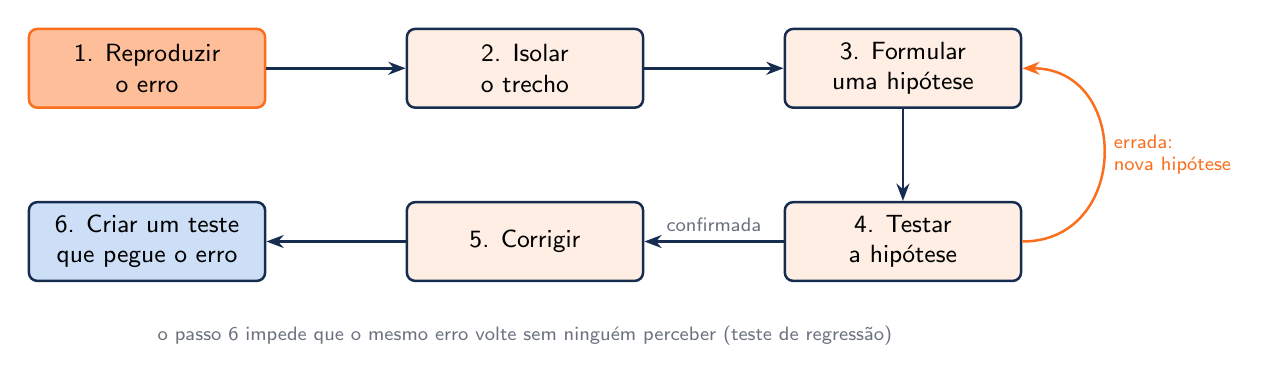
\begin{tikzpicture}
  \node[inicio] (rep) at (0, 0) {1. Reproduzir\\o erro};
  \node[passo] (iso) at (4.8, 0) {2. Isolar\\o trecho};
  \node[passo] (hip) at (9.6, 0) {3. Formular\\uma hipótese};
  \node[passo] (tes) at (9.6, -2.2) {4. Testar\\a hipótese};
  \node[passo] (cor) at (4.8, -2.2) {5. Corrigir};
  \node[fim] (reg) at (0, -2.2) {6. Criar um teste\\que pegue o erro};
  \draw[seta] (rep) -- (iso);
  \draw[seta] (iso) -- (hip);
  \draw[seta] (hip) -- (tes);
  \draw[seta] (tes) -- node[legenda, above] {confirmada} (cor);
  \draw[seta] (cor) -- (reg);
  \draw[seta, laranja] (tes.east) to[out=0, in=0, looseness=1.6]
    node[legenda, text=laranja, right, align=left] {errada:\\nova hipótese} (hip.east);
  \node[legenda, align=center] at (4.8, -3.4)
    {o passo 6 impede que o mesmo erro volte sem ninguém perceber (teste de regressão)};
\end{tikzpicture}
\end{document}
